\documentclass[11pt,a4paper]{article}
\usepackage[margin=1in]{geometry}
\usepackage{booktabs,graphicx,float,hyperref,xcolor,amsmath}
\usepackage[default]{sourcesanspro}
\hypersetup{colorlinks=true,linkcolor=blue,urlcolor=blue}
\title{Multivariate Weather Forecasting with RNNs\\\large LSTM, GRU, Sequence-to-Sequence, and Temporal Attention}
\author{Mohammad Torabi \\ 404422041}
\date{Course: Data Mining \\ Instructor: Dr. Hadi Farahani \\ August 2026}
\begin{document}
\maketitle
\begin{abstract}
This project forecasts temperature and relative humidity from the Jena Climate data at 6-, 24-, and 72-hour horizons. I compare persistence, direct LSTM, direct GRU, sequence-to-sequence LSTM, and an attention sequence-to-sequence model. My contribution is the attention ablation under the same sequence-to-sequence setup. Attention improves mean MAE over the matched Seq2Seq LSTM by 6.9\% at 6 hours and 15.9\% at 72 hours. However, persistence is still the strongest overall baseline in this one-epoch CPU run, so the neural results need more training before making a practical claim.
\end{abstract}

\section{Problem and Data}
The Jena Climate record contains 14 weather variables measured every 10 minutes. I keep every sixth row to make hourly data. The first 70\% of time is training data, the next 15\% is validation data, and the final 15\% is chronological test data. Missing wind values marked as $-9999$ are replaced using training medians, and all inputs are standardized from training statistics only.

Each model receives 72 past hourly readings and forecasts temperature ($T$) and relative humidity ($rh$) for the next 72 hours. I evaluate the 6-, 24-, and 72-hour positions. The chronological split is important because random splitting would leak future weather patterns into training.
\begin{figure}[H]\centering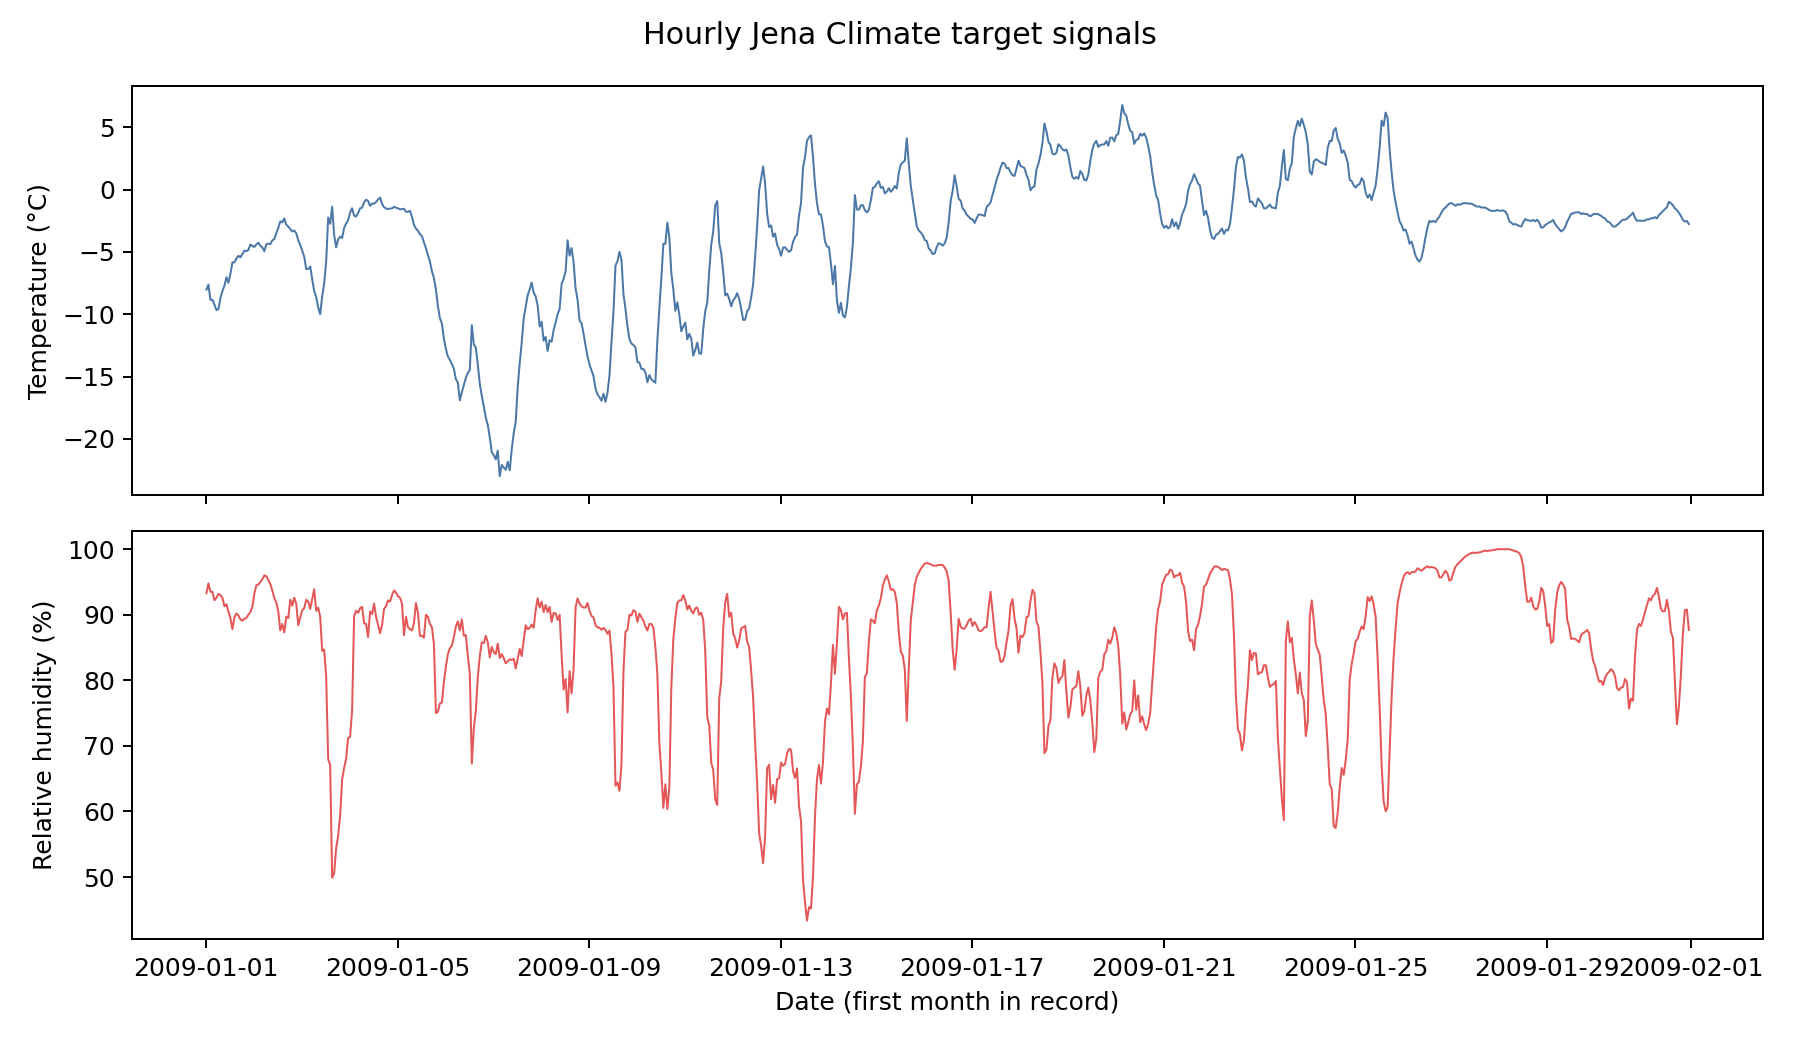
\includegraphics[width=.9\linewidth]{figures/target_timeseries.png}\caption{Hourly temperature and relative-humidity signals from the beginning of the record.}\label{fig:signals}\end{figure}
\begin{figure}[H]\centering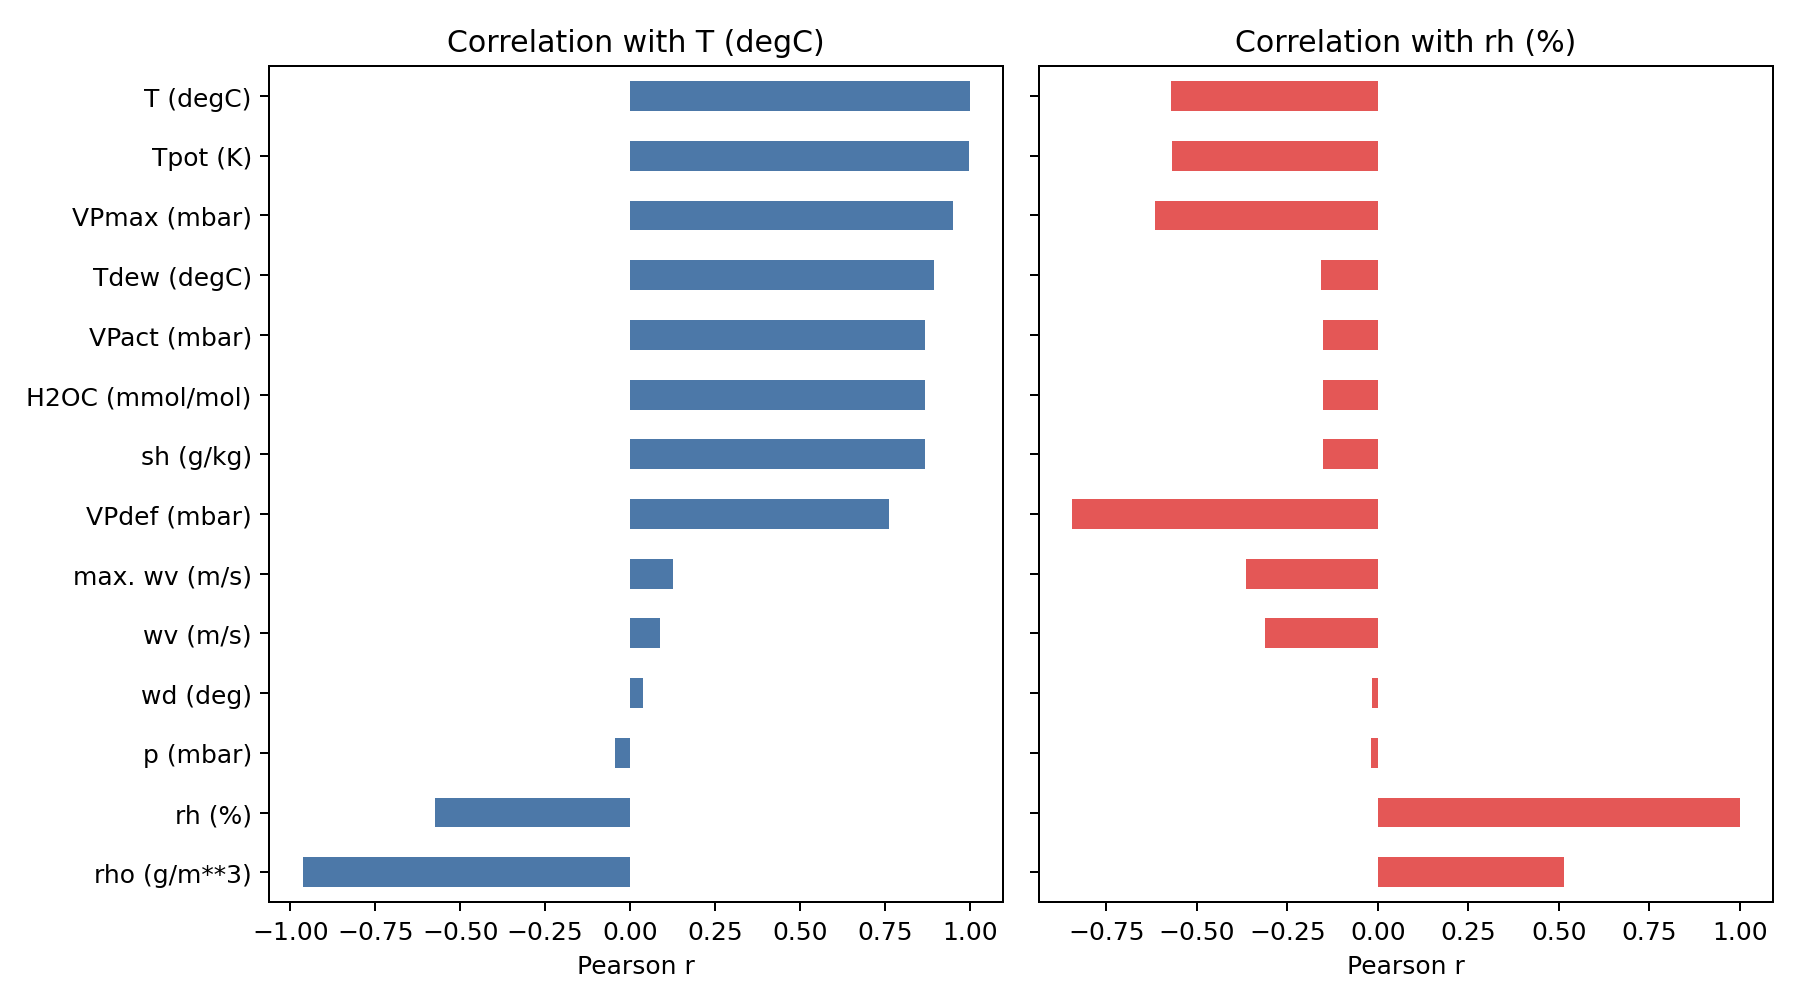
\includegraphics[width=\linewidth]{figures/correlations.png}\caption{Input-sensor correlations with the two forecast targets.}\label{fig:correlations}\end{figure}

\section{Method and Contribution}
Persistence repeats the last observed value. The direct LSTM and GRU encode the 72-hour input and use a linear head for the full forecast. Seq2Seq LSTM encodes the history and decodes a 72-step trajectory. The attention model adds dot-product temporal attention over encoder states at each decoding step.

All RNNs use hidden size 32, AdamW, batch size 1024, seed 42, and one training epoch. I use MAE and RMSE in the original physical units. My hypothesis was that attention would help the sequence-to-sequence model more at long horizons, because it can retrieve earlier daily-cycle and weather-regime information instead of relying only on the last encoder state.

\section{Real Results and Honest Analysis}
Table~\ref{tab:results} is regenerated from the saved \path{outputs/results.csv}. Among neural models, Attention Seq2Seq has the lowest mean MAE at 6 hours and GRU has the lowest mean MAE at 72 hours. Compared with the matched Seq2Seq LSTM, attention is better at both 6 and 72 hours, which supports part of my hypothesis. The improvement is larger at 72 hours (15.9\%) than at 6 hours (6.9\%).

At the same time, persistence has lower error than every neural model for the two targets at each displayed horizon in this saved run. For example, at 24 hours persistence has temperature MAE 2.498 and humidity MAE 9.815; the best neural temperature value is 3.379 from LSTM and the best neural humidity value is 10.792 from GRU. Therefore, the correct conclusion is not that attention solves this forecasting problem. The run is an ablation result, but one epoch is not enough to beat a strong recent-value baseline on this split.

\begin{table}[H]\centering\scriptsize
\caption{Saved test-set MAE and RMSE. Lower is better.}\label{tab:results}
\input{generated_results.tex}
\end{table}
\input{generated_summary.tex}
\begin{figure}[H]\centering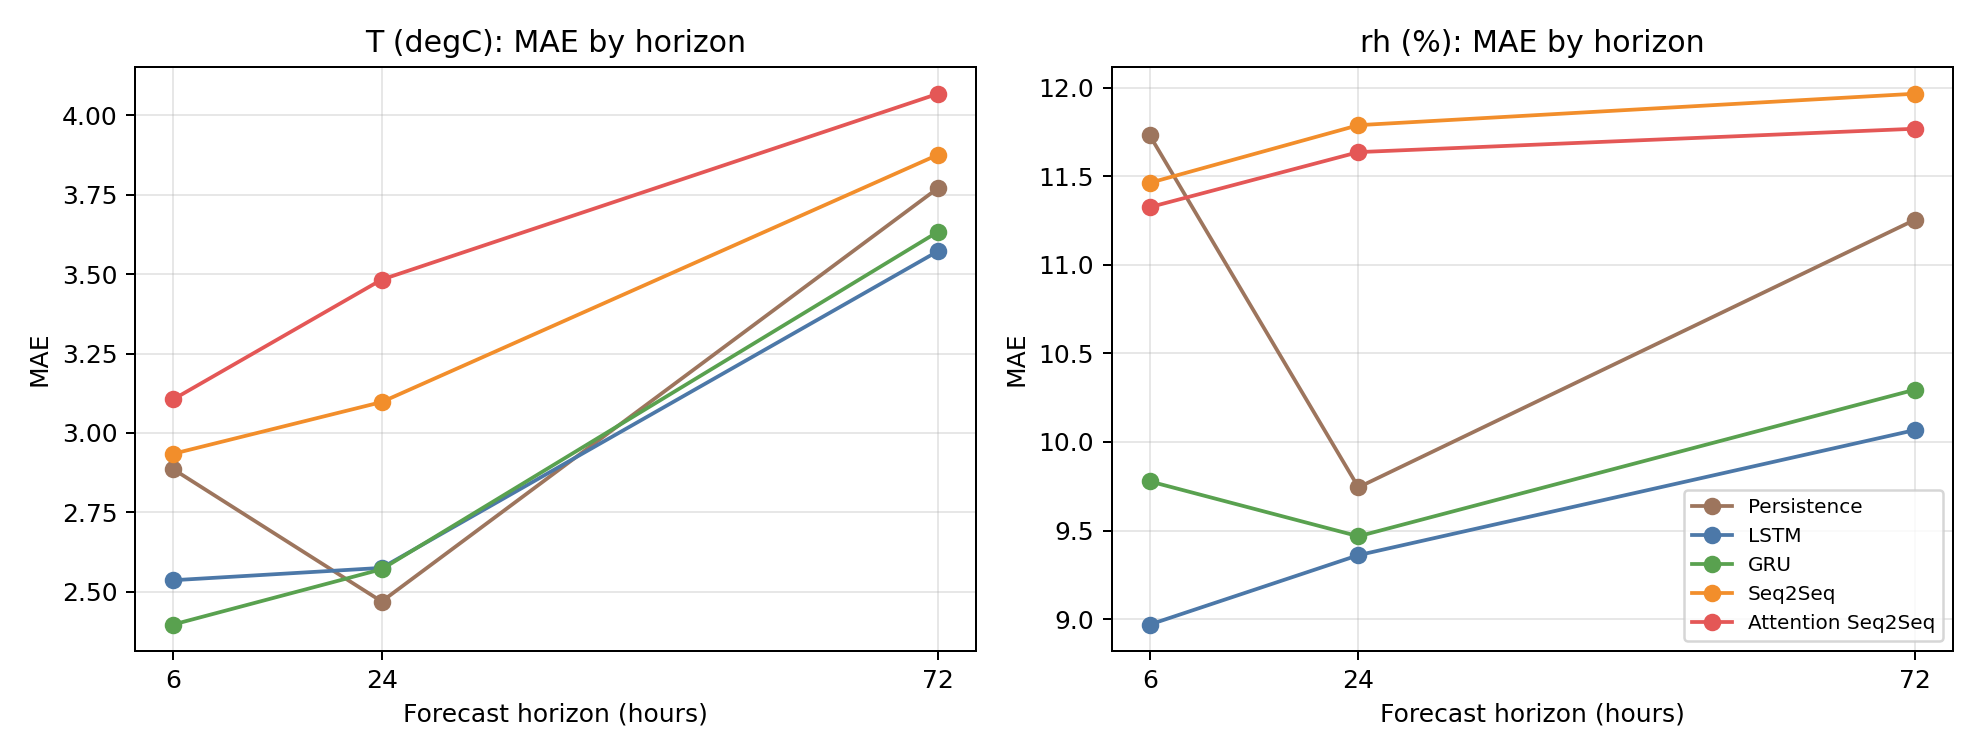
\includegraphics[width=\linewidth]{figures/mae_by_horizon.png}\caption{MAE by horizon for every saved model.}\label{fig:mae}\end{figure}
\begin{figure}[H]\centering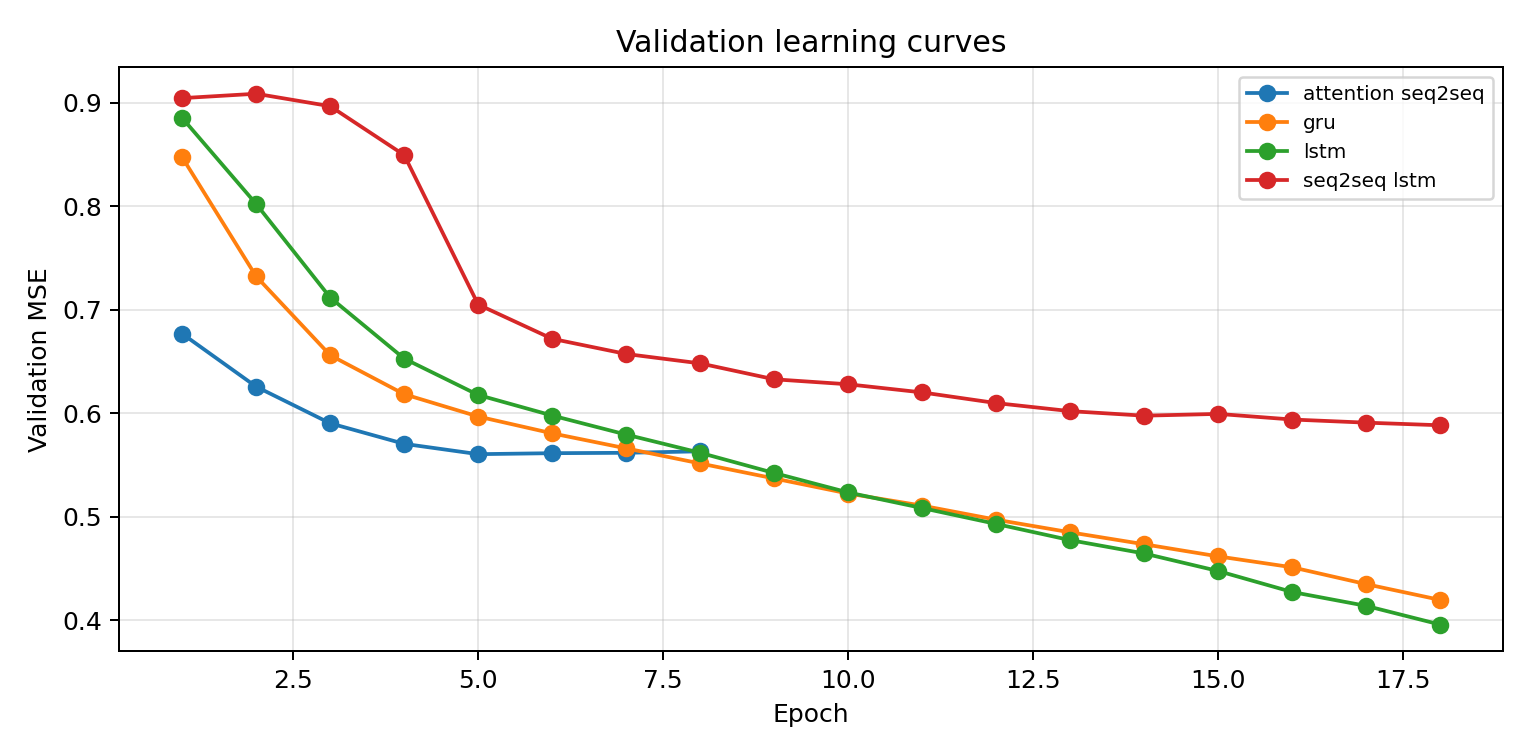
\includegraphics[width=.8\linewidth]{figures/learning_curves.png}\caption{One-epoch validation learning curves.}\label{fig:learning}\end{figure}

The forecast examples in Figure~\ref{fig:examples} also show why long horizons are difficult. When the weather changes quickly, small early errors can become larger later in the forecast. A longer training schedule, smaller batch size, repeated seeds, and tuning the models against validation performance are needed before comparing the final architectures.
\begin{figure}[H]\centering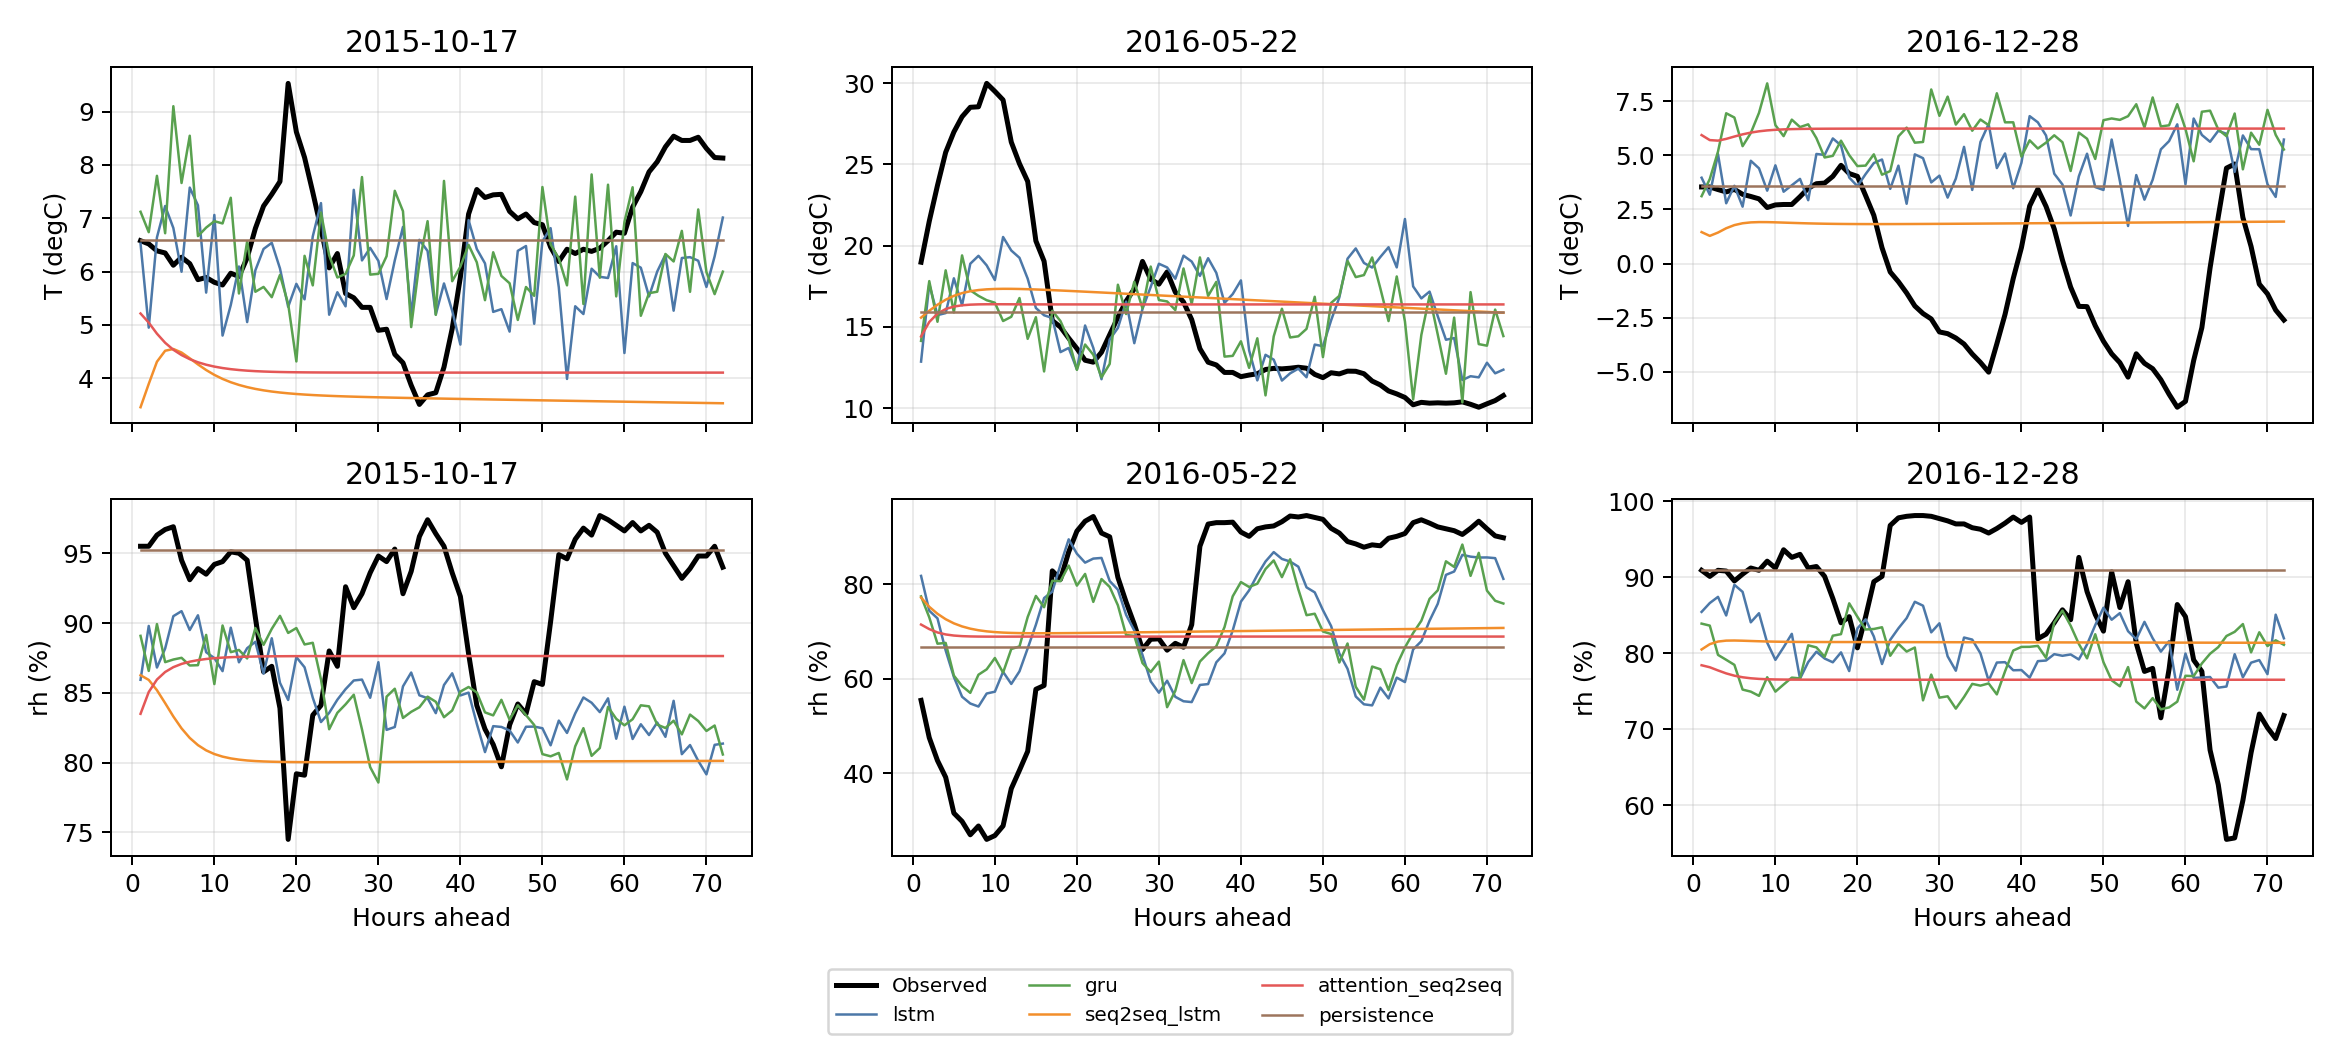
\includegraphics[width=\linewidth]{figures/forecast_examples.png}\caption{Saved chronological forecast examples.}\label{fig:examples}\end{figure}

\section{Discussion and Observation}
\subsection*{What should temporal attention look back at?}
I expect attention to use recent states during a rapid change, but also states around 24 hours earlier when the daily cycle is useful. My result is consistent with a larger long-horizon benefit against the matched Seq2Seq model, but it does not prove that the weights learned a meaningful meteorological pattern. I would inspect attention maps and repeat training before making this interpretation stronger.

\subsection*{Why retain the RNN sequential bias?}
An RNN updates a compact state step by step, which is a useful bias for a medium-size regularly sampled time series. A Transformer can connect distant times directly, but it normally requires more memory, positional choices, and enough data to learn this structure. For 72-hour windows and one station, I would first choose a small RNN when compute is limited. For longer histories or many stations, direct global interactions may be worth the cost.

\section{Limitations and Reproducibility}
The saved run uses only one epoch, so it is a verification experiment rather than a final optimized forecast system. It has one station and no uncertainty intervals. Run \path{python scripts/train.py}, then \path{python scripts/build_report_assets.py}, and compile this report to reproduce the metrics table and figures.
\end{document}
